\section{Afstandsbedømmelse - Praktisk del af jagtprøven)}

\begin{frame}
  \vspace{1.5em}
  \begin{center}
    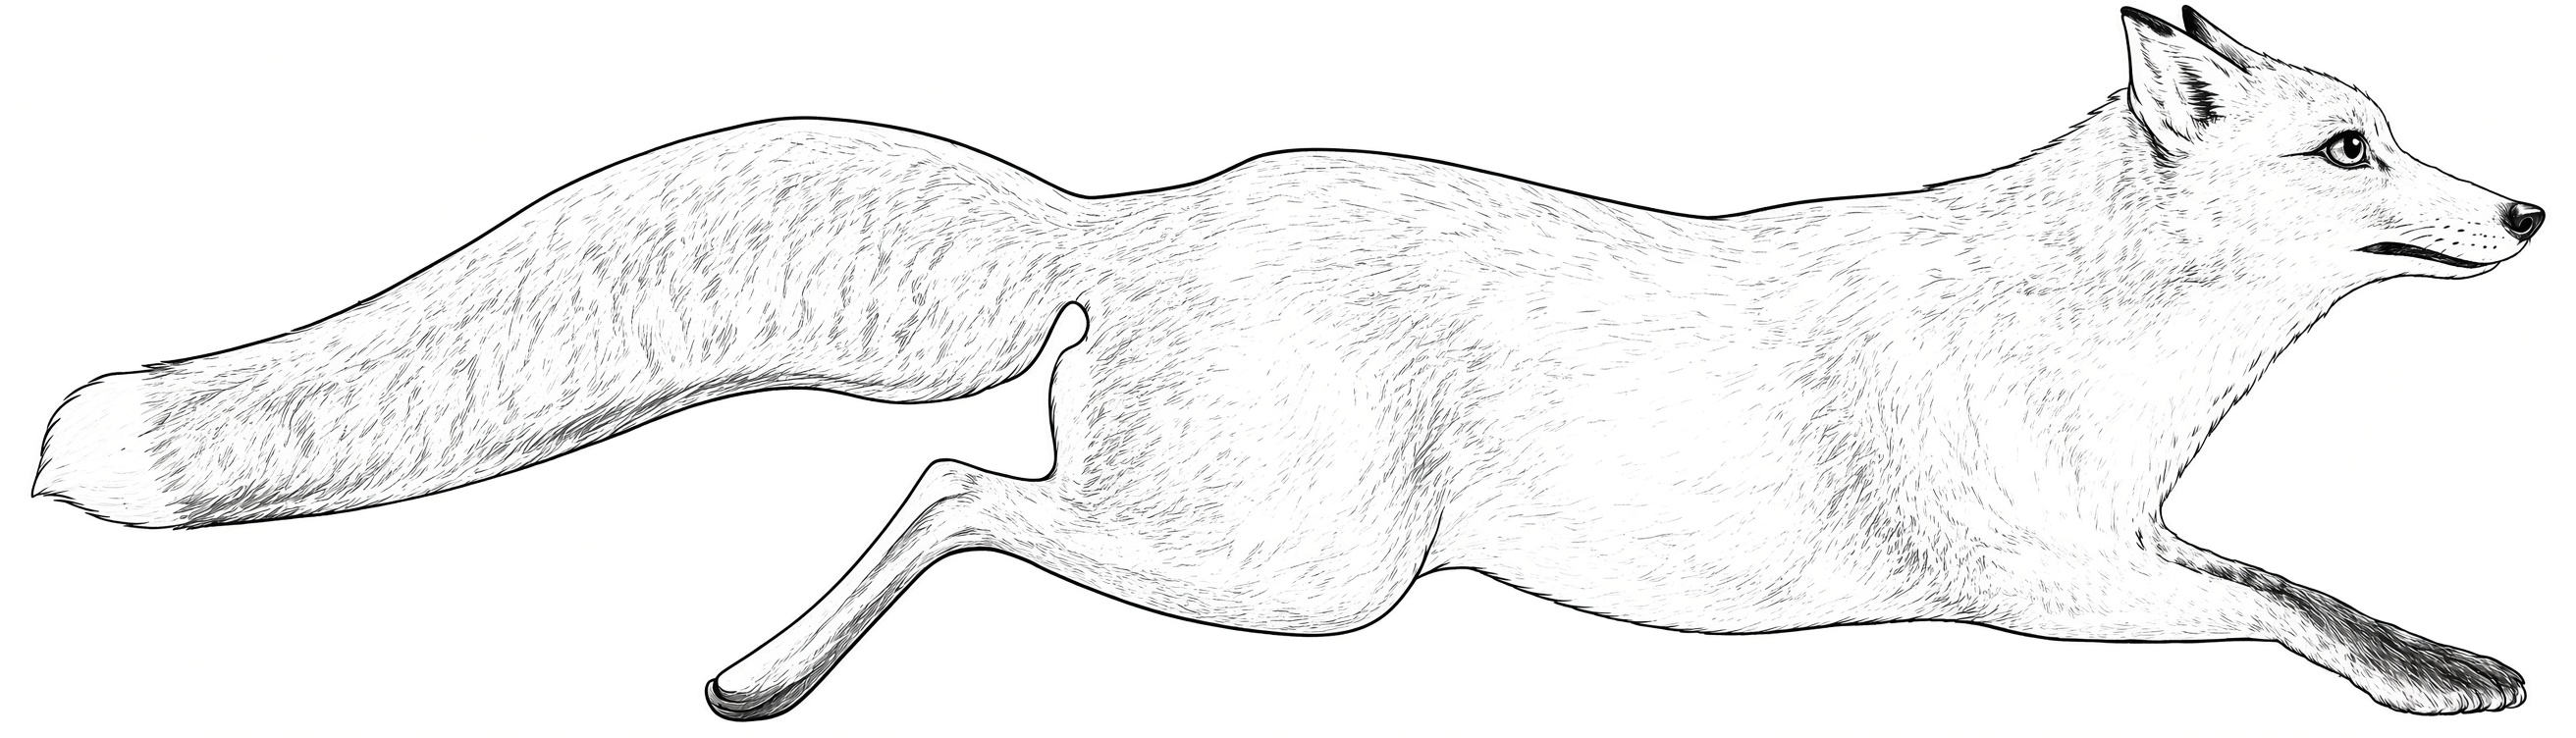
\includegraphics[width=12cm, height=2cm, keepaspectratio]{Billeder/Andet/Afstandsbedømmelse/afstandsbedømmelse.jpg}\\[1.2em]
    {\LARGE \textbf{Afstandsbedømmelse}}
    \vspace{1em}
    \\ En del af jagtprøven
    \\[0.9em]
    {\tiny\color{gray}
    CC BY 4.0 – kan frit anvendes, også kommercielt. Rettighederne må ikke skærpes.\\[0.05em]
    Udviklet af Aleksander Sønder, OSJAGTTEGN.DK}
  \end{center}
\end{frame}

% ========== AFSTANDSVURDERING ==========
\begin{frame}{Afstandsbedømmelse struktur}
  \tiny
  \setlength{\parskip}{0.35em}
  \RaggedRight

  \textbf{Sådan foregår afstandsbedømmelse}
  \begin{itemize}
    \itemsep0.15em
    \item Aspiranten skal vurdere afstanden ved \textbf{4 forskellige punkter}.
    \item Ved hvert punkt står \textbf{1 eller 2 vildtfigurer} efter den valgte afstandsserie.
    \item Der spørges om \textbf{1 figur ad gangen}.
    \item Figuren udpeges, og der spørges: \textit{``Er skudafstanden forsvarlig til \ldots?''}
    \item Herefter starter tidtagningen. Svarfristen er \textbf{5 sekunder}.
    \item Klart svar: enten JA el. NEJ \textbf{fejl}.
    \item Svar efter tiden tæller som \textbf{fejl}.
    \item Efter hvert punkt får aspiranten at vide, om svaret var korrekt.
  \end{itemize}

  \textbf{Krav til opstilling}
  \begin{itemize}
    \itemsep0.15em
    \item Punkterne placeres hensigtsmæssigt på den enkelte bane.
    \item Der må \textbf{ikke} bruges faste baner, så forløbet kan forudses.
    \item Mindst \textbf{1 fuglefigur} skal være hævet \textbf{2--4 m} over aspirantens niveau og så vidt muligt med himlen som baggrund.
    \item Samme afstandsserie bruges til samme prøvehold.
    \item Ved mistanke om snyd sættes en \textbf{ny serie} op.
    \item Afstandene skal måles før hver prøvedag med båndmål, målehjul eller laser.
  \end{itemize}

  \vspace{0.3em}
  \textbf{Beståkrav:} 5 ud af 6 afstande skal besvares korrekt.
\end{frame}

% ========== VILDTFIGURER: MAX OG PLACERING ==========
\begin{frame}{Vildtfigurer system, 3 klasser og 5 afstande}
  \vspace{-0.3em}
  \centering
  \scriptsize
  \setlength{\tabcolsep}{5pt}
  \renewcommand{\arraystretch}{1.25}

  \begin{tabular}{l c c l l}
    \toprule
    \textbf{Art} & \textbf{Billede} & \textbf{Max} & \textbf{Korrekt} & \textbf{Forkert} \\
    \midrule
    Gråand
      & 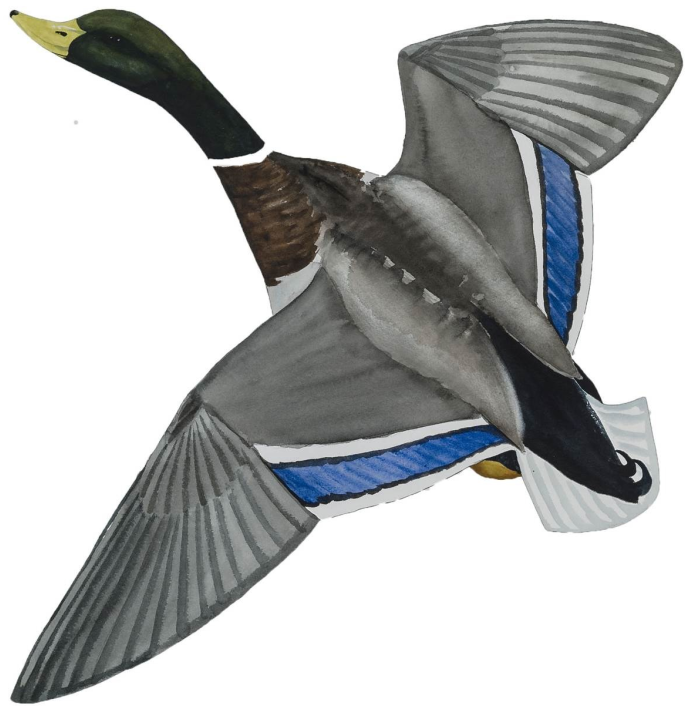
\includegraphics[height=0.9cm]{Billeder/Andet/Afstandsbedømmelse/gråand.png}
      & 30 m
      & 26 m (JA)
      & 38 m (NEJ) \\
    Hare
      & 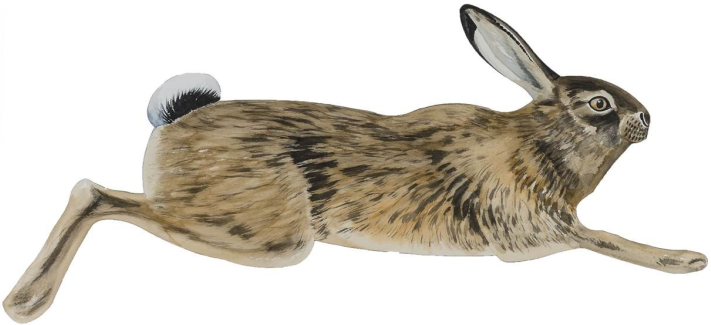
\includegraphics[height=0.9cm]{Billeder/Andet/Afstandsbedømmelse/hare.png}
      & 30 m
      & 26 m (JA)
      & 38 m (NEJ) \\
    Fasan
      & 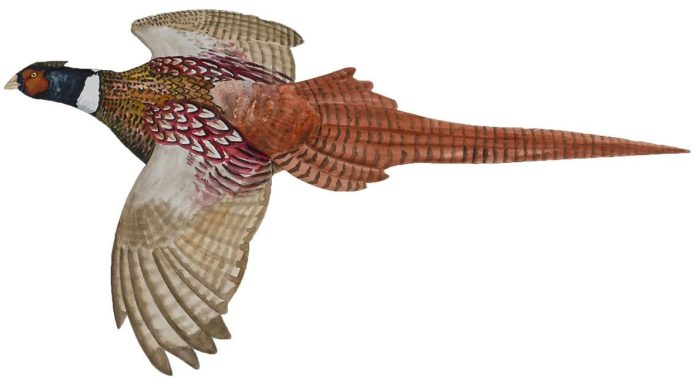
\includegraphics[height=0.9cm]{Billeder/Andet/Afstandsbedømmelse/fasan.png}
      & 30 m
      & 26 m (JA)
      & 38 m (NEJ) \\
    Ræv
      & 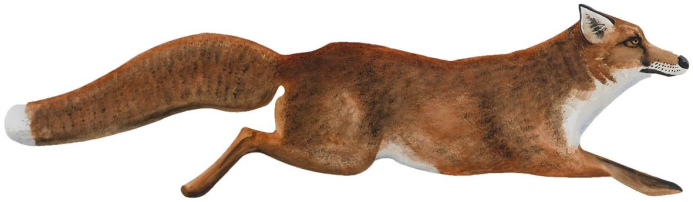
\includegraphics[height=0.9cm]{Billeder/Andet/Afstandsbedømmelse/ræv.png}
      & 25 m
      & 22 m (JA)
      & 32 m (NEJ) \\
    Grågås
      & 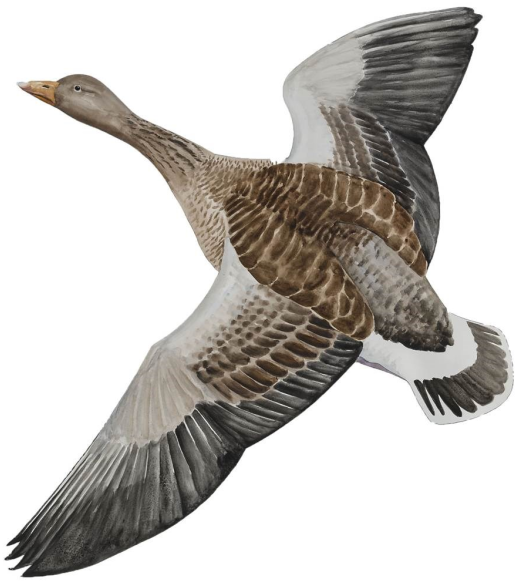
\includegraphics[height=0.9cm]{Billeder/Andet/Afstandsbedømmelse/grågås.png}
      & 25 m
      & 22 m (JA)
      & 32 m (NEJ) \\
    Råvildt
      & 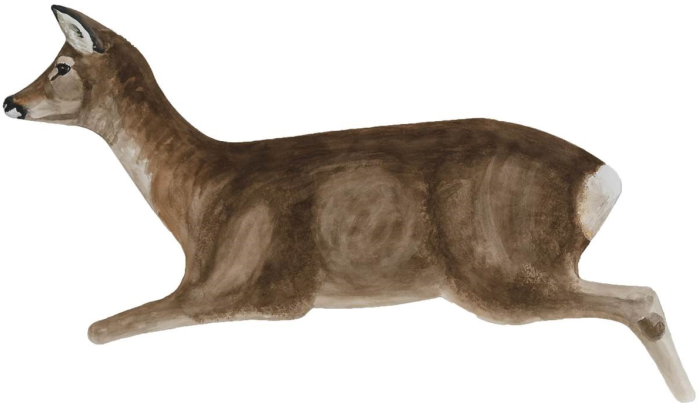
\includegraphics[height=0.9cm]{Billeder/Andet/Afstandsbedømmelse/råvildt.png}
      & 20 m
      & 17 m (JA)
      & 26 m (NEJ) \\
    \bottomrule
  \end{tabular}

  \vspace{0.8em}
  \tiny
  \textbf{JA} = inden for teoretisk max-skydeafstand \quad
  \textbf{NEJ} = længere end teoretisk max-skydeafstand
\end{frame}



% ========== SERIEPUNKTER ==========
\begin{frame}{Forskellige serier}
  \vspace{0.3em}
  \centering
  \footnotesize
  \begin{tabular}{lcccccccc}
    \toprule
    \textbf{Serie} & \textbf{1} & \textbf{2} & \textbf{3} & \textbf{4} & \textbf{5} & \textbf{6} & \textbf{7} & \textbf{8} \\
    \midrule
    Gråand (max.\ 30)   & 26 & 38 & 26 & 38 & 26 & 38 & 26 & 38 \\
    Ræv (max.\ 25)      & 22 & 32 & 22 & 32 & 22 & 32 & 22 & 32 \\
    Hare (max.\ 30)     & 26 & 26 & 26 & 26 & 38 & 38 & 38 & 38 \\
    Råvildt (max.\ 20)  & 17 & 17 & 26 & 26 & 17 & 17 & 26 & 17 \\
    Fasan (max.\ 30)    & 38 & 26 & 38 & 38 & 38 & 26 & 38 & 26 \\
    Grågås (max.\ 25)   & 32 & 22 & 32 & 22 & 22 & 32 & 32 & 22 \\
    \bottomrule
  \end{tabular}
\end{frame}